%
% teil1.tex -- Beispiel-File für das Paper
%
% (c) 2020 Prof Dr Andreas Müller, Hochschule Rapperswil
%
% !TEX root = ../../buch.tex
% !TEX encoding = UTF-8
%
\section{Grundbegriffe der Baustatik und Mechanik}
\label{elastomechanik:section:teil1}
\subsection{Begriffe}
\begin{description}	
	\item[\textbf{Druckkräfte:}] Druckkräfte sind Kräfte, die senkrecht auf die Oberfläche eines Körpers wirken und dabei eine Kompression bzw. Zusammenstauchung des Körpers verursachen. 
	Eine negative Normalkraft entspricht einer Druckkraft.
	
	\item[\textbf{Druckspannungen:}] Druckspannungen sind Spannungen, die im Inneren eines Materials entstehen, wenn Druckkräfte senkrecht auf die Oberfläche eines Körpers ausgeübt werden. 
	Sie bewirken eine Stauchung oder Kompression des Materials.
	Druckspannungen haben ein negatives Vorzeichen, da die Kräfte nach innen gerichtet sind.
	
	\item[\textbf{Elastizitätsmodul ($E$):}] Der Elastizitätsmodul (E-Modul) ist eine Materialkonstante, die die Steifigkeit eines Werkstoffs beschreibt. 
	Er gibt an, wie stark ein Material auf eine mechanische Spannung mit Dehnung reagiert. 
	Je grösser der Elastizitätsmodul, desto weniger verformt sich das Material unter einer gegebenen Belastung.
	Der Elastizitätsmodul wird definiert als:
	\begin{equation}
		E=
		\frac{\sigma}{\varepsilon}
	\end{equation}
	$\sigma$ = Spannung
	
	$\varepsilon$ = Dehnung
	
	\item[\textbf{Isotropie:}] Isotropie beschreibt eine Materialeigenschaft, bei der die mechanischen Eigenschaften in allen Raumrichtungen identisch sind. 
	Ein isotropes Material reagiert auf Belastungen unabhängig von der Belastungsrichtung stets gleich.
	In der linearen Elastizitätstheorie bedeutet Isotropie, dass das Materialverhalten vollständig durch zwei unabhängige Materialkonstanten beschrieben werden kann, etwa den Elastizitätsmodul ($E$) und die Poissonzahl ($\nu$).  
	Isotrope Annahmen vereinfachen die mathematische Modellierung deutlich und finden in der technischen Mechanik insbesondere bei homogenen Metallen, Glas und einigen Kunststoffen Anwendung \cite{elastomechanik:Isotropie}.
	
	\item[\textbf{Kinematische Gleichungen (Verzerrungsdefinition):}] Die kinematischen Gleichungen beschreiben den Zusammenhang zwischen den Verschiebungen $u_i$ eines Punktes im Raum und den daraus resultierenden Verzerrungen $\varepsilon_{ij}$. 
	Sie sind die Grundlage für die geometrische Beschreibung der Deformation in der Elastizitätstheorie. 
	Für kleine Verformungen gilt \cite{elastomechanik:Technische_Mechanik_2:Elastostatik}:
	\begin{equation}
		\varepsilon_{ij} = 
		\frac{1}{2} \left( \frac{\partial u_i}{\partial x_j} + \frac{\partial u_j}{\partial x_i} \right)
	\end{equation}
	Dabei ist:
	
		$u_i$ = Verschiebung in Richtung $i$
		
		$x_j$ = Raumkoordinate in Richtung $j$
		
	Diese Gleichungen stellen sicher, dass die Verzerrungen aus einem stetigen Verschiebungsfeld berechnet werden können.
	
	\item[\textbf{Normalkraft ($N$):}] Die Normalkraft ist eine Kraft, die senkrecht (normal) zur Querschnittsfläche eines Körpers oder Bauteils wirkt. 
	Sie entsteht durch Zug oder Druck entlang der Längsachse des Körpers und ist eine der wichtigsten Grundkräfte in der Technischen Mechanik und Statik.
	
	\item[\textbf{Normalspannungen ($\sigma_N$):}] Die Normalspannung ist eine Form der Spannung, die auftritt, wenn eine Kraft senkrecht (normal) zur Fläche eines Körpers wirkt. 
	Sie beschreibt den inneren Spannungszustand eines Materials bei Zug- oder Druckbelastung.
	
	\item[\textbf{Poissonzahl ($\nu$):}] Die Poissonzahl, auch bekannt als Querkontraktionszahl, ist eine materialabhängige Konstante, die das Verhältnis zwischen der Querdehnung und der Längsdehnung eines Körpers unter Zug- oder Druckbelastung beschreibt.
	Sie ist definiert als
	\begin{equation}
		\nu=
		-\frac{\varepsilon_{quer}}{\varepsilon_{laengs}}
	\end{equation}
	$\varepsilon_{quer}$ = Dehnung senkrecht zur Belastungsrichtung
	
	$\varepsilon_{laengs}$ = Dehnung in Belastungsrichtung
	
	\item[\textbf{Schubmodul ($\mu$) oder ($G$):}] Der Schubmodul ist eine mechanische Materialkonstante, die beschreibt, wie steif ein Material gegenüber Scherkräften ist.
	Scherkräfte (auch Schubkräfte) sind Kräfte, die parallel zur Fläche eines Körpers wirken. 
	Bei isotropen Materialien wird es folgend berechnet:
	\begin{equation}
		\mu = 
		\frac{E}{2(1 + \nu)} =
		G
	\end{equation}
	\begin{figure} [h]
		\centering
		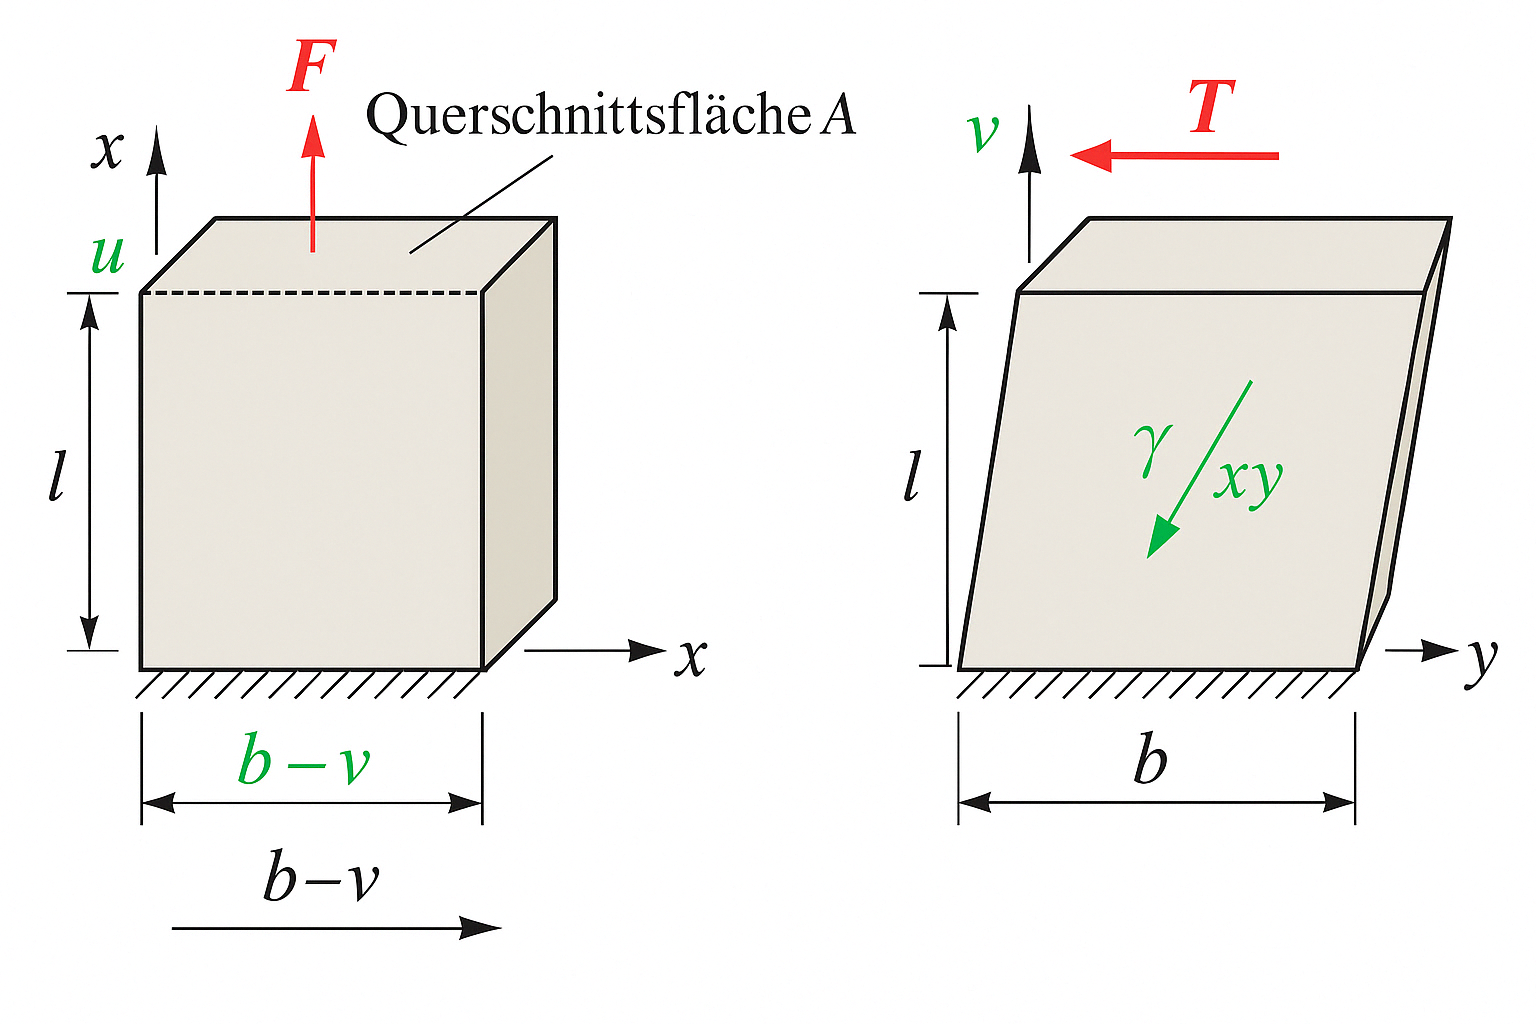
\includegraphics[width=\textwidth]{papers/elastomechanik/images/teil1/Zugverformung_Schubverformung.png}
		\caption{Die linke Abbildung zeigt eine Normalverzerrung infolge axialer Belastung, die rechte Abbildung eine Schubverzerrung infolge tangentialer Beanspruchung.}
		\label{fig:Zugverformung_Schubverformung}
	\end{figure}
	\item[\textbf{Spannung ($\sigma$):}] Die Spannung beschreibt die innere Kraftverteilung in einem Material, die infolge externer Belastungen (wie Zug, Druck oder Scherung) entsteht. 
	Sie gibt an, welche Kraft pro Flächeneinheit innerhalb eines Körpers wirkt.
	
	\item[\textbf{Spannungtensor ($\sigma_{ij}$):}] Der Spannungstensor (auch Cauchy-Spannungstensor genannt) beschreibt die Verteilung der inneren Spannungen im Material. 
	Der erste Index	i gibt die Richtung der Flächennormalen an, der zweite Index j die Richtung der Spannungswirkung. 
	Er ist in der Regel symmetrisch und wird als 3×3-Matrix notiert \cite{elastomechanik:Grundlagen_der_Elastizitaetstheorie}:
	\begin{equation}
	\boldsymbol{\sigma} =
	\begin{bmatrix}
		\sigma_{xx} & \sigma_{xy} & \sigma_{xz} \\
		\sigma_{yx} & \sigma_{yy} & \sigma_{yz} \\
		\sigma_{zx} & \sigma_{zy} & \sigma_{zz}
	\end{bmatrix}
	\end{equation}
	Da der Spannungstensor symmetrisch ist (für reine Elastizität), gilt:
	\begin{equation}
		\sigma_{ij} = 
		\sigma_{ji}
	\end{equation}
	\item[\textbf{Verzerrung ($\varepsilon$):}] Die Verzerrung (auch Dehnung genannt) beschreibt die relative Änderung der Form oder Länge eines Körpers infolge einer äusseren Belastung. 
	Sie ist ein massloser Wert, da sie ein Verhältnis zweier Längen ist.
	Die Normalverrung wird berechnet mit
	\begin{equation}
		\varepsilon 
		= \frac{\Delta L}{L_0}
	\end{equation}
	$\varepsilon$ = Verzerrung
	
	$\Delta L$ = Längenänderung
	
	$\L_0$ = ursprüngliche Länge des Körpers
	
	\item[\textbf{Verzerrungstensor ($\varepsilon_{ij}$):}] Der Verzerrungstensor beschreibt die Verformung (Dehnung und Scherung) eines Körpers infolge äusserer Belastungen in drei Raumrichtungen. 
	Er erfasst nicht nur Längenänderungen (Normalverzerrungen), sondern auch Winkeländerungen (Schubverzerrungen) und stellt somit die vollständige lokale Verformung eines Materials im Raum dar.
	Die Verzerrungstensor wird über die Ableitungen des Verschiebungsfeldes definiert als
	\begin{equation}
		\varepsilon_{ij} = 
		\frac{1}{2} \left( \frac{\partial u_i}{\partial x_j} + \frac{\partial u_j}{\partial x_i} \right)
	\end{equation}
	wobei er in drei Raumdimensionen die Form einer symmetrischen 3×3-Matrix annimmt:
	\begin{equation}
	\boldsymbol{\varepsilon} =
	\begin{bmatrix}
		\varepsilon_{xx} & \varepsilon_{xy} & \varepsilon_{xz} \\
		\varepsilon_{yx} & \varepsilon_{yy} & \varepsilon_{yz} \\
		\varepsilon_{zx} & \varepsilon_{zy} & \varepsilon_{zz}
	\end{bmatrix}
	\end{equation}
	\item[\textbf{Zugkraft:}] Die Zugkraft ist eine Kraft, die längs zur Achse eines Körpers wirkt und diesen in Richtung Verlängerung belastet. 
	Sie verursacht Zugverformungen im Material.
	
	\item[\textbf{Zugspannungen:}] Die Zugspannung ist die innere Spannung, die durch eine Zugkraft im Material erzeugt wird. 
	Sie wirkt senkrecht zur Querschnittsfläche des Körpers und beschreibt die Kraft pro Flächeneinheit, mit der das Material dem Zug widersteht.
\end{description}

\subsection{Materialgesetzlichkeiten}
\begin{description}	
	\item[\textbf{Elastizitätsgesetz (Hookesches Gesetz):}] Das Hookesche Gesetz stellt im eindimensionalen Fall den linearen Zusammenhang zwischen Spannung $\sigma$ und Dehnung $\varepsilon$ durch die Beziehung 
	\begin{equation}
		\sigma = 
		E \cdot \varepsilon
	\end{equation}
	 her.
	 
	 Wobei $E$ der Elastizitätsmodul des Materials ist \cite{elastomechanik:Kontinuumsmechanik}.
	 \item[\textbf{Gleichgewichtsbedingungen:}] Diese bilden den zweiten Bestandteil der Herleitung und folgen in der Regel auf das Materialgesetz. 
	 Sie stellen sicher, dass im Inneren des Körpers keine resultierende Kraft wirkt, also mechanisches Gleichgewicht herrscht.
	 Lokal formuliert ergibt sich:
	 \begin{equation}
	 	\frac{\partial \sigma_{ij}}{\partial x_j} + f_i =
	 	0
	 \end{equation}
	 Dabei bezeichnet $\sigma_{ij}$ die Spannungskomponenten und $f_i$ die Komponenten der Volumenkraft pro Einheit Volumen. 
	 Die Gleichung fordert, dass die Summe der inneren Spannungsänderungen und der äusseren Volumenkräfte in jedem Punkt verschwindet. Sie gilt für jeden Punkt des Körpers und bildet die Grundlage für die statische Beschreibung des Spannungsfeldes \cite{elastomechanik:Grundlagen_der_Elastizitaetstheorie}.
	 \item[\textbf{Isotropes Materialverhalten:}] Für isotrope Materialien (die in alle Richtungen die gleichen mechanischen Eigenschaften haben) reicht die Beschreibung mit zwei Materialkonstanten $\lambda$ und $\mu$ aus.
	 \begin{equation}
	 	\sigma_{ij} = 
	 	\lambda \cdot \delta_{ij} \cdot \varepsilon_{kk} + 2\mu \cdot \varepsilon_{ij},
	 \end{equation}
	$\sigma_{ij}$ = Spannungstensor (Komponenten der Spannung in Richtung $i$ auf der Fläche senkrecht zu Richtung $j$)
	$\varepsilon_{ij}$ = Dehnungstensor (Komponenten der Verzerrung)
	
	$\varepsilon_{kk}$ = Spur des Verzerrungstensors, also
	\begin{equation}
		\varepsilon_{11} + \varepsilon_{22} + \varepsilon_{33}
	\end{equation}
	das ist die Volumendehnung \cite{elastomechanik:Grundlagen_der_Elastizitaetstheorie}.
	 $\delta_{ij}$ = Kronecker-Delta 
	 
	 $\lambda_{,\mu}$ = Lame’sche Konstanten
	 
	 Viele Metalle, wie beispielsweise Stahl, können näherungsweise als isotrope Materialien betrachtet werden.
	 
	 \vspace{0.5em}
	 Bei \textbf{anisotropen Materialien} hingegen sind die mechanischen Eigenschaften richtungsabhängig. 
	 Die Spannungs-Dehnungs-Beziehung erfordert in diesem Fall einen allgemeinen Elastizitätstensor vierter Stufe:
		 \begin{equation}
	 		\sigma_{ij} = 
	 		C_{ijkl} \cdot \varepsilon_{kl}
		 \end{equation}
	 Die Anzahl der unabhängigen Komponenten dieses Tensors kann, je nach Symmetrieeigenschaften, zwischen 21 und 81 liegen. 
	 Ein typisches Beispiel für anisotropes Verhalten ist Holz, dessen Steifigkeit von der Faserrichtung abhängt.
	 Für unsere Arbeit wird die Herleitung des anisotropen Materialverhaltens nicht thematisiert, da sie den Rahmen dieser Seminararbeit sprengen würde.
	 
	 \item[\textbf{Lame’sche Konstanten ($\lambda_{,\mu}$):}] Die Lame'schen Konstanten werden die Konstanten $\lambda$ und $\mu$ bezeichnet. 
	 Die sind zwei materialabhängige Parameter, die das mechanische Verhalten eines isotropen elastischen Materials vollständig beschreiben.
	 Die Lame’sche Konstante ($\lambda$) lässt sich aus dem Elastizitätsmodul und der Poissonzahl wie folgt berechnen \cite{elastomechanik:Grundlagen_der_Elastizitaetstheorie}:
	 \begin{equation}
	 	\lambda = 
	 	\frac{E \cdot \nu}{(1 + \nu)(1 - 2\nu)}
	 \end{equation}
	 $\mu$ = Schubmodul
	 
	 $\lambda$ = steht in Verbindung mit der Volumenverformung
	 
	 \item[\textbf{Materialverhaltenseigenschaften:}] Für ideal elastisches Verhalten gilt:
	 \begin{enumerate}
	 	\item Dehnung verschwindet vollständig bei Entlastung.
	 	
	 	\item Der Energieinhalt ist vollständig reversibel.
	 	
	 	\item Das Verhalten ist unabhängig von der Geschwindigkeit der Belastung.
	 	
	 	\item Es existiert eine eindeutige Beziehung zwischen Spannung und Dehnung
	 \end{enumerate}
	 \item[\textbf{Reziproke Form (für Verzerrungen aus Spannungen):}] Die reziproke Form des Hooke’schen Gesetzes beschreibt den linearen Zusammenhang zwischen Spannung und Verzerrung bei isotropen Materialien durch die Gleichung
	 \begin{equation}
	 	\varepsilon_{ij} = 
	 	\frac{1+\nu}{E} \cdot \sigma_{ij} - \frac{\nu}{E} \cdot \sigma_{kk} \cdot \delta_{ij}
	 \end{equation}
	 wobei die Verzerrung aus der direkten Spannung und der Spur des Spannungstensors unter Berücksichtigung des Elastizitätsmoduls und der Poissonzahl berechnet wird \cite{elastomechanik:Grundlagen_der_Elastizitaetstheorie}.
\end{description}
